\documentclass{beamer}
\usepackage{tikz,xcolor}
\usetikzlibrary{trees,arrows}
\usepackage{amsmath}
\mode<presentation> {

% The Beamer class comes with a number of default slide themes
% which change the colors and layouts of slides. Below this is a list
% of all the themes, uncomment each in turn to see what they look like.

%\usetheme{default}
%\usetheme{AnnArbor}
%\usetheme{Antibes}
%\usetheme{Bergen}
%\usetheme{Berkeley}
%\usetheme{Berlin}
%\usetheme{Boadilla}
%\usetheme{CambridgeUS}
%\usetheme{Copenhagen}
%\usetheme{Darmstadt}
%\usetheme{Dresden}
%\usetheme{Frankfurt}
%\usetheme{Goettingen}
%\usetheme{Hannover}
%\usetheme{Ilmenau}
%\usetheme{JuanLesPins}
%\usetheme{Luebeck}
\usetheme{Madrid}
%\usetheme{Malmoe}
%\usetheme{Marburg}
%\usetheme{Montpellier}
%\usetheme{PaloAlto}
%\usetheme{Pittsburgh}
%\usetheme{Rochester}
%\usetheme{Singapore}
%\usetheme{Szeged}
%\usetheme{Warsaw}

% As well as themes, the Beamer class has a number of color themes
% for any slide theme. Uncomment each of these in turn to see how it
% changes the colors of your current slide theme.

%\usecolortheme{albatross}
%\usecolortheme{beaver}
%\usecolortheme{beetle}
%\usecolortheme{crane}
%\usecolortheme{dolphin}
%\usecolortheme{dove}
%\usecolortheme{fly}
%\usecolortheme{lily}
%\usecolortheme{orchid}
%\usecolortheme{rose}
%\usecolortheme{seagull}
%\usecolortheme{seahorse}
%\usecolortheme{whale}
%\usecolortheme{wolverine}

%\setbeamertemplate{footline} % To remove the footer line in all slides uncomment this line
%\setbeamertemplate{footline}[page number] % To replace the footer line in all slides with a simple slide count uncomment this line

%\setbeamertemplate{navigation symbols}{} % To remove the navigation symbols from the bottom of all slides uncomment this line
}

\usepackage{graphicx} % Allows including images
\usepackage{booktabs} % Allows the use of \toprule, \midrule and \bottomrule in tables
\usepackage{latexsym}
\usepackage{amsmath}
\usepackage{amssymb}
\usepackage{amsthm}
\usepackage{bm}
\usepackage{float}
\usepackage{array}
\usepackage{multirow}

\def\dfrac#1#2{{\displaystyle\frac{#1}{#2}}}
\def\bd#1{\boldsymbol{#1}}
\def\mva{{\mathcal{VA}}}
\def\mpass{{\mathcal{PASS}}}
\def\mpv{{\mpass(\mva)}}
\def\mcl{{\mathcal{CL}}}
\def\mcls{{\mathcal{CLS}}}
\def\mlit{{\mathcal{LIT}}}
\def\msat{{\mathcal{SAT}}}
\def\musat{{\mathcal{USAT}}}
\def\pmva{{\pmb{\mathcal{VA}}}}
\def\pmlit{{\pmb{\mathcal{LIT}}}}
\def\pmpv{{\pmb{\mpass(\mva)}}}
\def\pmcl{{\pmb{\mathcal{CL}}}}
\def\pmcls{{\pmb{\mathcal{CLS}}}}
\def\var{{\rm var}}
\def\bvar{{\bf var}}

\def\q{{\quad}}
\def\d{{\rm d}}


%----------------------------------------------------------------------------------------
%	TITLE PAGE
%----------------------------------------------------------------------------------------

\title[Short title]{Boolean Satisfiability Solving Solvers} % The short title appears at the bottom of every slide, the full title is only on the title page

\author{Pengyun Ji} % Your name
\institute[SWAN] % Your institution as it will appear on the bottom of every slide, may be shorthand to save space
{
Swansea University \\ % Your institution for the title page
\medskip
\textit{jipengyun@hotmail.com} % Your email address
}
\date{\today} % Date, can be changed to a custom date

\begin{document}

\begin{frame}
\titlepage % Print the title page as the first slide
\end{frame}

\begin{frame}
\frametitle{Overview} % Table of contents slide, comment this block out to remove it
Basic Concepts
\begin{itemize}
\item Definitions
\item Satisfiability and Unsatisfiability
\item Conjunctive normal form(CNF)
\end{itemize}
Algorithms
\begin{itemize}
\item Davis-Putnam Algorithm
\item Backtracking Search
\item Boolean Constraint Propagation
\end{itemize}
\end{frame}

%----------------------------------------------------------------------------------------
%	PRESENTATION SLIDES
%----------------------------------------------------------------------------------------

%------------------------------------------------
%\section{First Section} % Sections can be created in order to organize your presentation into discrete blocks, all sections and subsections are automatically printed in the table of contents as an overview of the talk
%------------------------------------------------
%\subsection{Subsection Example} % A subsection can be created just before a set of slides with a common theme to further break down your presentation into chunks

\begin{frame}
\frametitle{Definitions}
\begin{itemize}
\item Variables \\
Let $\pmva$ be a set of  \textbf{variables}.\\
$\mva$ may be empty;\\
$\mva$ may be finite;\\
$\mva$ may be infinite (ie $\mva = \mathbb{N}$ or $\mva = \mathbb{R}$).
\\~\\
\item Literals \\
\textbf{literal} is a variable or a negated variable.\\
we use $\pmlit(\pmva)$ to define the set of literals over $\mva$.
\\~\\
\item Clause \\
We denote $\pmcl(\pmva)$ as the set of finite subsets $C\subseteq \mlit(\mva)$. \\
\textbf{Clauses} are the elements of $\mcl(\mva)$ over $\mva$.

\end{itemize}
\end{frame}

%------------------------------------------------
\begin{frame}
\frametitle{Definitions}
\begin{itemize}
\item Clause-sets \\
We denote $\pmcls(\pmva)$ as the set of subsets $F\subseteq \mcl(\mva)$.\\
\textbf{Clause-sets} are the elements of $\mcls(\mva)$.\\~\\
In other words, a \textbf{clause-set} is a set of \textbf{clauses}, and a \textbf{clause} is a set of literals:
\begin{eqnarray*}
&(a\vee b) \wedge (\neg c\vee d) \rightsquigarrow \left\{ \; \{a,b\}, \{\overline{c}, d\} \; \right\}& \\
& a\wedge b\wedge (\neg a \vee \neg b \vee \neg c) \rightsquigarrow \left\{ \; \{a\},\{b\}, \{\overline{a}, \overline{b}, \overline{c}\} \; \right\}&
\end{eqnarray*}
\item Partial assignments \\
Denote $\pmpv$ as the set of all maps of assignments $\varphi : V \to \{ 0, 1 \}$ for finite subsets $V\subseteq \mva$.\\
\textbf{partial assignments} are the elements of $\mpv$ over $\mva$.
\end{itemize}
\end{frame}

%---------------------------------------------------
\begin{frame}
\frametitle{Satisfiability and Unsatisfiability}
A clause-set $F$ is \textbf{satisfiable} iff there is an assignment $\varphi$ of truth-values to variables such that in every clause $C \in F$ there is at least one literal $x \in C$ getting truth value 1, i.e., $\varphi(x) = 1$, while otherwise $F$ is \textbf{unsatisfiable}.\\
Therefore we could define:
\begin{align*}
\pmb{\msat(\mva)} := \{ F & \in \mcls(\mva)| \\
& \; \exists \; \varphi \in \mpass(\mva) : \varphi(F) = 1 \}
\end{align*}
\begin{align*}
& \pmb{\musat(\mva)} := \mcls(\mva) \;\backslash\; \msat(\mva) = \\
& \;\; \{F\in \mcls(\mva) \mid \forall\; \varphi \in \mpass(\mva) : \varphi(F) \neq 1\}.
\end{align*}

\end{frame}

%------------------------------------------------------
\begin{frame}
\frametitle{Conjunctive normal forms (CNF)}
\textbf{conjunctive normal form (CNF)} is a special case of propositional formula, restricted representation of formula as\\
Literals: Variables or Negated Variables\\
Clauses: Disjunctions of Literals\\
CNF Formulas: Conjunctions of Clauses\\~\\
Examples:
\begin{eqnarray*}
&(a\vee b) \wedge (\neg a \vee c) \wedge (b\vee \neg c)& \\
&a\wedge b \wedge c& \\
\end{eqnarray*}
Basically, the meaning of the \textbf{SAT} problem is:\\
Given a conjunctive normal form F, decide whether F is satisfiable or not.
\end{frame}


%-----------------------------------------------------------

\begin{frame}
\frametitle{Properties of CNF}
Pure Variable
\begin{itemize}
\item The literals appears only positive or negative in a CNF formula.
\end{itemize}
Empty Clause
\begin{itemize}
\item If a CNF formula has some Clause without Literals
\item Then the CNF formula is $\pmb\musat$
\end{itemize}
Trivial Formula
\begin{itemize}
\item If a CNF formula has no Clause
\item Or every variable is pure
\item Then the CNF formula is $\pmb{\msat}$
\end{itemize}
Goal: Determine satisfaction by reducing CNF formula to one of
\begin{itemize}
\item Empty Clause (ie $\pmb\musat$), or
\item Trivial Formula (ie $\pmb\msat$)
\end{itemize}

\end{frame}

%------------------------------------------------

\begin{frame}
\frametitle{Resolution}
Two CNF clauses that contain a variable x in opposite polarity imply a new
CNF clause that contains all literals except x and $\neg x$ \\~\\

Example: For any $A,B$ and variable $x$, the formula
\[
(A \vee x) \wedge (B \vee \neg x)
\]
is {\it equivalent} to the formula $(A \vee B)$.\\~\\
we can say that $x$ is a {\bf pivot} variable.
\end{frame}


\begin{frame}
\frametitle{General Resolution}
Generally, for any $A_i,B_j$ and variable $x$, the formula
\[
\bigwedge_i
(A_i \vee x) \wedge
\bigwedge_j
(B_j \vee \neg x)
\]
is {\it equivalent} to the formula
\[
\bigwedge_{i,j}
(A_i \vee B_j )
\]
The pivot variable $x$ is {\bf eliminated} by resolution.

\end{frame}

\begin{frame}
\frametitle{Davis-Putnam Algorithm}
Algorithm
\begin{itemize}
\item Select a pivot variable x to perform resolution on.
\item Retain only the newly added clauses and the ones not containing x.
\item Repeat until $\pmb\msat$ or $\pmb\musat$.
\end{itemize}
Examples:
\begin{enumerate}[\quad1.]
\item[1.] $(x_1 \vee x_2 \vee x_3 ) \wedge (x_2 \vee \neg x_3 \vee x_5 ) \wedge (\neg x_2 \vee x_4 )$
\item[2.] $(x_1 \vee x_2 ) \wedge (x_1 \vee \neg x_2 ) \wedge (\neg x_1 \vee x_3 ) \wedge (\neg x_1 \vee \neg x_3 )$
\end{enumerate}
\end{frame}


\begin{frame}
\frametitle{Backtracking Search}
\begin{itemize}
\item Choose a variable $x$, set to true
\item Eliminate all clauses where $x$ appears
\item Remove all literals $\neg x$
\item Recurse on remaining clauses
\item Backtrack if a contradiction is found
\end{itemize}
\end{frame}

\begin{frame}
\frametitle{Backtracking Search}
\vspace*{1cm}
\hspace*{7mm}
\begin{minipage}{.22\textwidth}
\begin{flushleft}
$(a'+b+c)$

$(a+c+d)$

$(a+c+d')$

$(a+c'+d)$

$(a+c'+d')$

$(b'+c'+d)$

$(a'+b+c')$

$(a'+b'+c)$

\end{flushleft}
\end{minipage}
\begin{minipage}{.6\textwidth}
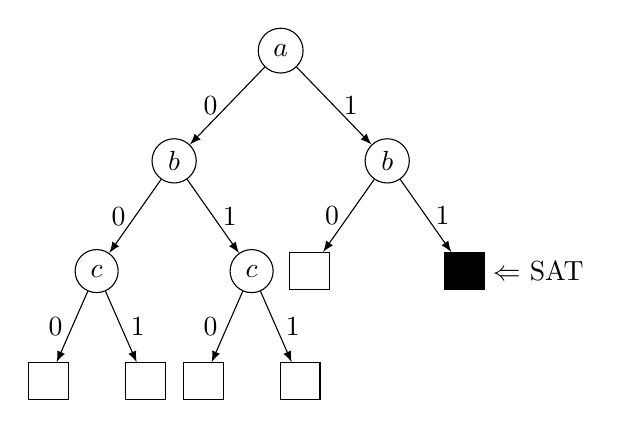
\begin{tikzpicture}[level 3/.style={sibling distance=5em},level 2/.style={sibling distance=8em},level 1/.style={sibling distance=11em}, level distance = 2cm, scale=0.7,edge from parent/.style={draw,-latex}, every circle node/.style={draw},level 4/.style={level distance =2cm}]
  \node(root)[circle] {$a$}
child { node[circle,inner sep=2.8pt] {$b$}
child { node[circle] {$c$}
child { node[rectangle,draw] {\color{white}$-$}
edge from parent
node[left] {$0$}
}
child { node[rectangle,draw] {\color{white}$-$}
edge from parent
node[right] {$1$}
}
edge from parent
node[left] {$0$}
}
child { node[circle] {$c$}
child { node[rectangle,draw] {\color{white}$-$}
edge from parent
node[left] {$0$}
}
child { node[rectangle,draw] {\color{white}$-$}
edge from parent
node[right] {$1$}
}
edge from parent
node[right] {$1$}
}
edge from parent
node[left] {$0$}
}
child {node[circle,inner sep=2.8pt]  {$b$}
child {node[rectangle,draw] {\color{white}$-$}
edge from parent
node[left] {$0$}
}
child {node[rectangle,draw,fill,black] {\color{black}$-$}node[right]{~~$\Leftarrow $ SAT}
edge from parent
node[right] {$1$}
}
edge from parent
node[right] {$1$}
};
\end{tikzpicture}
\end{minipage}
\end{frame}


\begin{frame}
\frametitle{Boolean Constraint Propagation}
Unit Clause Rule
\begin{itemize}
\item If an unsatisfied clause has one unassigned literal
\item Then that literal must be \textbf{TRUE} in any SAT assignment
\item Repeat applying unit clause rule
\item Until no unit clause remains.
\end{itemize}
Example
\begin{itemize}
\item Formula $(x_1 \vee \neg x_2 \vee x_3)\wedge(x_2 \vee \neg x_3)\wedge(\neg x_1 \vee \neg x_3)$
\item Assignment $x_1 = T, x_2 = T$
\item The last clause is a unit clause
\item Any SAT assignment must set $\neg x_3 = T$ $(i.e. x_3 = F)$
\end{itemize}
\end{frame}

\begin{frame}
\frametitle{Boolean Constraint Propagation}
\vspace*{5mm}
\begin{minipage}{.28\textwidth}
\begin{tabular}{c@{~$\vee$~}c@{~$\vee$~}c}
$\neg x_1$   & $x_2$ & $ x_3$\\
$x_1 $ &$x_3  $ &$x_4$\\
$x_1 $ &$ x_3  $ &$\neg x_4$\\
$x_1 $ &$\neg x_3$ &$   x_4$\\
$x_1 $ &$\neg x_3$ &$ \neg  x_4$\\
$\neg x_2 $ &$\neg x_3 $ &$  x_4$\\
$\neg x_1  $ &$x_2 $ &$\neg x_3$\\
$\neg x_1 $ &$\neg x_2 $ &$ x_3$\\
\end{tabular}
\end{minipage}
\begin{minipage}{.7\textwidth}
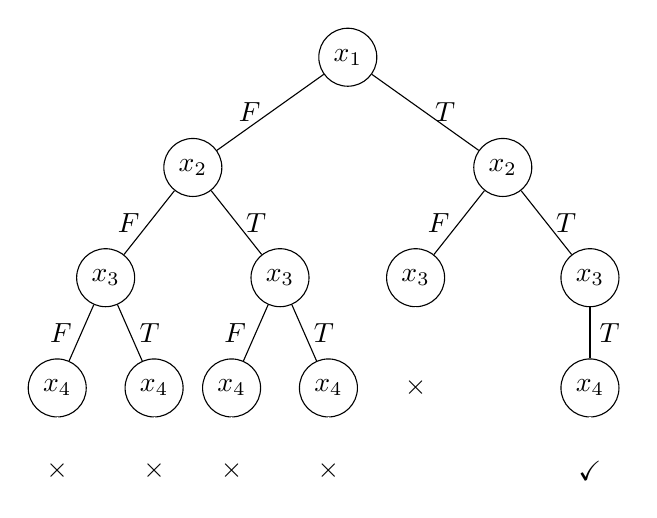
\begin{tikzpicture}[level 3/.style={sibling distance=5em},level 2/.style={sibling distance=9em},level 1/.style={sibling distance=16em}, level distance=2cm,scale=0.7,level 4/.style={level distance =1.5cm}]
  \node(root)[circle,draw] {$x_1$}
child { node[circle,draw] {$x_2$}
child { node[circle,draw] {$x_3$}
child { node[circle,draw] {$x_4$}
child[white] { node[black] {$\times$}}
edge from parent
node[left] {$F$}
}
child { node[circle,draw] {$x_4$}
child[white] { node[black] {$\times$}}
edge from parent
node[right] {$T$}
}
edge from parent
node[left] {$F$}
}
child { node[circle,draw] {$x_3$}
child { node[circle,draw] {$x_4$}
child[white] { node[black] {$\times$}}
edge from parent
node[left] {$F$}
}
child { node[circle,draw] {$x_4$}
child[white] {node[black] {$\times$}}
edge from parent
node[right] {$T$}
}
edge from parent
node[right] {$T$}
}
edge from parent
node[left] {$F$}
}
child {node[circle,draw]  {$x_2$}
child {node[circle,draw] {$x_3$}
child[white] { node[black] {$\times$}}
edge from parent
node[left] {$F$}
}
child {node[circle,draw] {$x_3$}
child {node[circle,draw] {$x_4$}
child[white] { node[black] {$\checkmark$}}
edge from parent
node[right] {$T$}
}
edge from parent
node[right] {$T$}
}
edge from parent
node[right] {$T$}
};
\end{tikzpicture}
\end{minipage}
\end{frame}

\end{document} 
